Iptables es un programa que proporciona una interfaz de usuario para configurar Netfilter, que es el subsistema presente en el kernel de Linux para filtrado y manipulación de paquetes. Casi cualquier firewall de terceros que podemos descargar e instalar en Linux, como UFW o Firestarter, no son más que front-ends para Iptables.\\

Iptables es usado para crear y administrar reglas que proporcionan, entre otras cosas, capacidad para manipular los paquetes, control de la traducción NAT y seguimiento de conexiones. Iptables es un firewall de los llamados 'stateful', ya que mantiene el control de las conexiones establecidas por nuestro PC.

\section{Estructura y funcionamiento de iptables}
Iptables permite escribir \textbf{reglas} para control y manipulación de paquetes. Estas reglas se agrupan en \textbf{cadenas}, que a su vez pertenecen a una de las \textbf{tablas} presentes. \\

Las tablas disponibles son las siguientes:
\begin{itemize}
\item \textbf{Filter}, la tabla por defecto, provee comandos para filtar y aceptar o rechazar paquetes.
\item \textbf{Nat}, provee comandos para modificar la forma en que la máquina hace la traducción de direcciones.
\item \textbf{Mangle}, permite la modificación de los encabezamientos de los paquetes.
\item \textbf{Security}, proporciona reglas de control de acceso.
\item \textbf{Raw}, contiene herramientas para el seguimiento de conexiones.
\end{itemize}

Cada una de las tablas tiene diferentes cadenas, a las que añadiremos nuestras reglas:

\begin{longtable}{l | c}
\textbf{Tabla} \ \ \ & \textbf{Cadenas}\\\hline
\multirow{3}{*}{\textbf{filter}} & INPUT\\
& FORWARD\\
& OUTPUT\\\hline
\multirow{4}{*}{\textbf{NAT}} & PREROUTING\\
& INPUT\\
& OUTPUT\\
& POSTROUTING\\
\end{longtable}

\begin{longtable}{l | c}
\textbf{Tabla} & \textbf{Cadenas}\\\hline
\multirow{5}{*}{\textbf{mangle}} & PREROUTING\\
& INPUT\\
& FORWARD\\
& OUTPUT\\
& POSTROUTING\\\hline
\multirow{3}{*}{\textbf{security}} & INPUT\\
& FORWARD\\
& OUTPUT\\\hline
\multirow{2}{*}{\textbf{raw}} & PREROUTING\\
& OUTPUT\\
\end{longtable}

Para comprender bien el funcionamiento de Iptables debemos pensar desde el punto de vista de las cadenas en lugar de las tablas. El kernel de Linux procesa los paquetes en un orden que se corresponde con las cadenas. En esta imagen podemos ver las etapas por las que pasan los paquetes:

\begin{figure}[H]
    \centering
    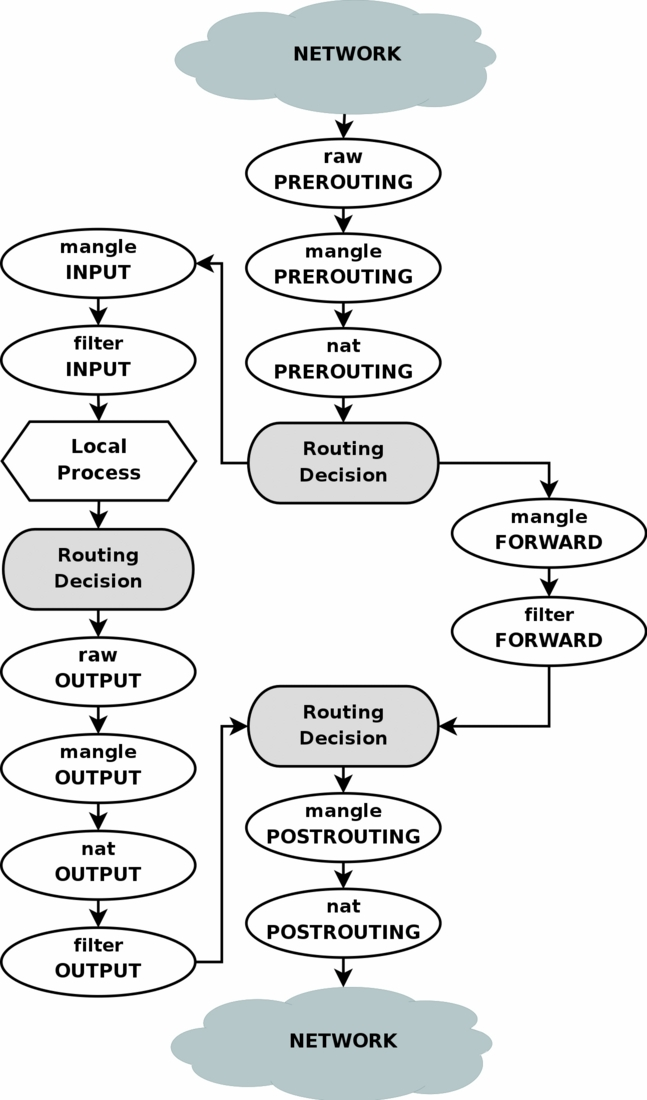
\includegraphics[width=0.55\textwidth]{iptables/00.jpg}
\end{figure}

Hay tres posibilidades diferentes según el camino que sigan los datos:

\begin{enumerate}[label=\bfseries\arabic*.]
\item \textbf{Paquetes destinados a nuestra máquina}

Cuando un paquete entra por una interfaz, inmediatamente se compara con las reglas que tengamos en la cadena PREROUTING, en el orden indicado en la imagen: primero las que están en la tabla \textit{raw}, luego las que están en la tabla \textit{mangle} y por último las que están en la tabla \textit{nat}. En este momento el paquete puede ser modificado. Por ejemplo, podemos cambiar la IP de destino y mandarlo a otro sitio, de manera que no será procesado por nuestro sistema. Se recomienda no usar nunca la cadena PREROUTING para filtrar, ya que en determinadas situaciones los paquetes no son filtrados correctamente.

Después, se toma la decisión de enrutamiento, con lo que se sigue el camino que vemos en la imagen hacia la izquierda. Se compara primero con la cadena INPUT de las tablas que la contienen. En este momento es cuando se filtran y modifican los paquetes. Finalmente se entrega al proceso local para que lo use.\\

\item \textbf{Paquetes generados por nuestra máquina}

Cuando el paquete se ha generado, se decide el enrutamiento y se elige qué dirección de origen usar y la interfaz por la que se va a enviar. Luego se compara con las reglas presentes en la cadena OUTPUT de las diferentes tablas. Con ellas podemos filtrar (tabla \textit{filter}) y cambiar las direcciones de origen y destino (tabla \textit{nat}), entre otras cosas.

Posteriormente se vuelve enrutar, ya que podríamos haber modificado el paquete, y se compara con las reglas de la cadena POSTROUTING. Finalmente se envía a la interfaz adecuada para que sea transmitido.\\

\item \textbf{Paquetes destinados a otro host}

En este caso el paquete entra y se compara con las reglas de la cadena PREROUTING, como hemos explicado antes, y luego se enruta. Si resulta que va dirigido a otro host, se compara con las reglas de la cadena FORWARD, en el orden indicado. Aquí podemos filtrar paquetes (tabla \textit{filter}) y modificarlos (tabla \textit{mangle}). Luego se vuelve a enrutar y se le aplican las reglas de la cadena POSTROUTING.

\end{enumerate}



\section{El comando iptables}

Veamos unos cuantos ejemplos para comprender la sintaxis:

\begin{lstlisting}
iptables -t nat -L
iptables -L
iptables -t nat -L PREROUTING
\end{lstlisting}

El primer comando muestra las reglas presentes en la tabla \textit{nat}. La tabla por defecto es \textit{filter}, por lo tanto se usará ésta siempre que no se especifque otra: el segundo ejemplo mostrará todas las reglas presentes en \textit{filter}. Se puede añadir el nombre de una cadena después para que solo muestre las reglas contenidas en ella.

\begin{figure}[H]
    \centering
    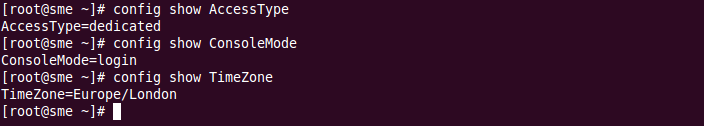
\includegraphics[width=\textwidth]{iptables/01.png}
\end{figure}

\begin{lstlisting}
iptables -t mangle -F INPUT
\end{lstlisting}

Borra todas las reglas de la cadena INPUT de la tabla \textit{mangle}. Si se omite el nombre de la tabla, se utilizará \textit{filter}. Si se omite el nombre de la cadena, se borrarán las reglas de todas las cadenas.\\

\begin{lstlisting}
iptables -t filter -P INPUT DROP
\end{lstlisting}

Cambia la política por defecto de la cadena INPUT de la tabla \textit{filter} a DROP. Los paquetes que se hayan comparado con todas las reglas de esta cadena y no se hayan encontrado con una orden ACCEPT serán rechazados.\\

\begin{lstlisting}
iptables -t nat -N miCadena
\end{lstlisting}

Crea una nueva cadena definida por el usuario, llamada \textit{miCadena}, en la tabla \textit{nat}. Estas cadenas deben ser llamadas desde las 5 originales, más adelante veremos cómo.

\subsection{Añadiendo reglas}

El comando básico para añadir una regla a una cadena de una tabla es

\begin{lstlisting}
iptables -t tabla -A CADENA descripición
\end{lstlisting}

La descripción de una regla se especifica escribiendo el valor de varios parámetros. Los parámetros disponibles son:

\begin{longtable}{p{0.21\textwidth} | p{0.7\textwidth}}
\textbf{Parámetro} & \textbf{Descripción}\\\hline
\lstinline!-p! \textit{protocolo} & Especifica el protocolo. Puede ser \textit{tcp}, \textit{udp} o \textit{icmp}, entre otros. Se puede usar un símbolo de exclamación, !, delante del protocolo para invertir la búsqueda.\\\hline
\lstinline!-s! \textit{IP/máscara} & Especificación del origen. Puede ser un nombre de host en lugar de una dirección IP. Se pueden poner varias separadas por coma. Se puede usar ! para invertir la búsqueda.\\\hline
\lstinline!-d! \textit{IP/máscara} & Dirección IP o nombre de host del destino.\\\hline
\lstinline!-m! \textit{parámetros} & Con \lstinline!-m! o \lstinline!--match! podemos dar condiciones más detalladas del paquete. Si las cumple, se ejecutará la acción en la opción \lstinline!-j!. Más abajo se dará una lista con los parámetros disponibles.\\\hline
\lstinline!-j! \textit{target} & Especifica qué hacer cuando el paquete cumple todas las condiciones establecidas en la regla. Los targets básicos son REJECT, DROP, ACCEPT y LOG. Algunos aceptan opciones extra. También se puede poner el nombre de una cadena personalizada, con lo que se pasará a comparar el paquete con todas las reglas de esa cadena.\\\hline
\lstinline!-i! \textit{interfaz} & Nombre de la inerfaz desde la que se ha recibido un paquete. Slo disponible en las cadenas INPUT, FORWARD y PREROUTING. Se puede usar ! al principio para revertir la búsqueda, o + al final como carácter comodín.\\\hline
\lstinline!-o! \textit{interfaz} & Nombre de la interfaz por la que el paquete va a ser enviado. Solo disponible en las cadenas FORWARD, OUTPUT y POSTROUTING. Se puede usar ! al principio para revertir la búsqueda, o + al final como carácter comodín.\\
\end{longtable}

Con la opción \lstinline!-m! debemos usar lo que se llaman \textbf{módulos} de filtrado. Cada módulo tiene un nombre y acepta diferentes opciones, que se pueden escribir en la misma línea. Algunos de ellos son:

\begin{longtable}{p{0.13\textwidth} | p{0.29\textwidth} | p{0.49\textwidth}}
\textbf{Módulo} &  \textbf{Opciones} & \textbf{Descripción}\\\hline
\lstinline!state! & \lstinline!--state! \textit{estado} & Comprueba el estado de conexión de ese paquete. El estado puede ser INVALID (no hay ninguna conexión conocida asociada a ese paquete), NEW (el paquete ha empezado una nueva conexión) y ESTABLISHED (el paquete está asociado a una conexión conocida, que ya ha enviado paquetes en ambos sentidos), entre otros.\\\hline
\lstinline!limit! & \lstinline!--limit! \textit{núm/ud\_tiempo} \quad \lstinline!--limit-burst! \textit{número} & La regla en la que está \lstinline!limit! se comprobará como máximo una vez en el intervalo de tiempo que le digamos. \lstinline!/s, /m, /h, /d! para segundos, minutos, horas y días. \lstinline!--limit-burst! marca el número de veces que se permiten antes de que el límite sea efectivo. Después de una regla con \lstinline!limit! se suele usar una con DROP, para descartar el resto de paquetes.\\\hline
\lstinline!tcp! & \lstinline!--sport! \textit{puerto[:puerto]} \lstinline!--dport! \textit{puerto[:puerto]} \hspace{2cm} \lstinline!--tcp-flags! \textit{flags} \textit{flags}
\lstinline!--syn! & Se pueden usar estas opciones directamente detrás de \lstinline!-p tcp! en una regla. Permite filtrar un paquete según su puerto de origen y destino (se pueden usar rangos), y según su tipo, dependiendo de las flags TCP que tenga. El primer parámetro en \lstinline!--tcp-flags! es para las flags que deben ser examinadas y el segundo para las que deben estar activadas, es decir las que estén en el primer parámetro y no en el segundo deberán estar sin activar. \lstinline!--syn! es equivalente a \lstinline!--tcp-flags SYN,RST,ACK,FIN SYN!\\
\end{longtable}

\newpage
Veamos algunos ejemplos sencillos de reglas:\\

\begin{lstlisting}
iptables -A INPUT -s 192.168.0.0/24 -j DROP
\end{lstlisting}

Descarta los paquetes que vengan desde la red 192.168.0.0/24 por cualquier interfaz. La diferencia entre los targets DROP y REJECT es que este último envía de vuelta un mensaje ICMP de destino inalcanzable (podemos cambiar este mensaje con la opción \hspace{0.7cm} \lstinline!--reject-with!), mientras que DROP lo bloquea sin más.\\

\begin{lstlisting}
iptables -A INPUT -i eth0 -p tcp -s 192.168.0.0/24 --dport 22 -m state NEW, ESTABLISHED -j ACCEPT
iptables -A OUTPUT -o eth0 -p tcp --sport 22 -m state --state ESTABLISHED -j ACCEPT
\end{lstlisting}

Permite todo el tráfico SSH que provenga de la red 192.168.0.0/24, siempre que haya iniciado la conexión otro host (esto último depende de la política por defecto que hayamos puesto en OUTPUT, suponemos que es DROP).\\

\begin{lstlisting}
iptables -t nat -A POSTROUTING -o eth0 -j MASQUERADE
iptables -A FORWARD -i eth0 -o eth1 -m state --state RELATED,ESTABLISHED -j ACCEPT
iptables -A FORWARD -i eth1 -o eth0 -j ACCEPT
\end{lstlisting}

Estas son las reglas necesarias para hacer traducción de direcciones. eth0 sería la interfaz externa y eth1 la interna. La primera regla es para que nuestra máquina enmascare el tráfico que sale hacia el exterior, es decir, que haga la traducción de direcciones para que parezca que el paquete ha sido enviado por ella. La segunda es para permitir todo el tráfico hacia las máquinas de la red interna, siempre que hayamos iniciado nosotros la comunicación. Está en la cadena FORWARD de la tabla \textit{filter}, con lo cual en el momento de comprobar esta regla ya se ha hecho el enrutamiento y la dirección de destino será una de nuestra red interna. La tercera regla sirve para permitir todo el tráfico desde nuestra red interna al exterior.

%BIBLIOGRAFIAA
%http://www.thegeekstuff.com/2011/06/iptables-rules-examples/
%https://help.ubuntu.com/community/IptablesHowTo
%http://gr8idea.info/os/tutorials/security/iptables8.html
%https://www.digitalocean.com/community/tutorials/iptables-essentials-common-firewall-rules-and-commands
%
